\section{Problem 2}
\textit{Using the FDTD matlab code given at the course, design a Yagi-Uda antenna that has a gain of at least 6 dBi at 850 Mhz.}


We followed the design diagram for a Yagi-Uda antenna of three elements found on-line and shown in \figref{fig:wiki_yagi_antenna}.

\begin{figure}[!h]
  \centering
  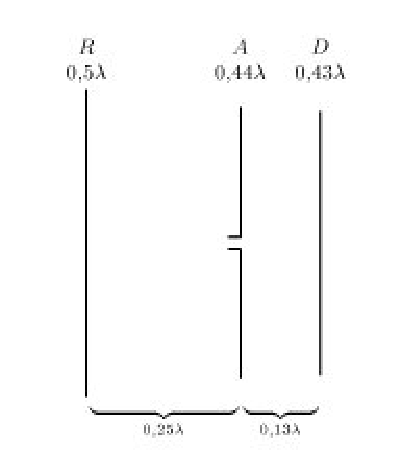
\includegraphics[width=10cm]{wiki_yagi_antenna.eps}
  \caption{Figure showing the angles involved in the dipole inclination and rotation (WRITE SOURCE)}
  \label{fig:wiki_yagi_antenna}
\end{figure}

Since the antenna should have a required gain of 6 dBi at 850 Mhz, our wavelength of interest is $\lambda = \SI{0.352}{\meter}$. Given that wavelength, since we wanted to have an accurate FDTD simulation, we set the cell size to $\SI{0.01}{\meter}$. The literature recommends to use a cell size of at least a tenth of a wavelength, with the chosen value we were sure that we were fulfilling that requirement.

The simulation geometry is shown in the \figref{fig:3_element_yagi-uda_geometry} and the simulation parameters are shown in \tref{tab:antenna_param}

\begin{figure}[!h]
  \centering
  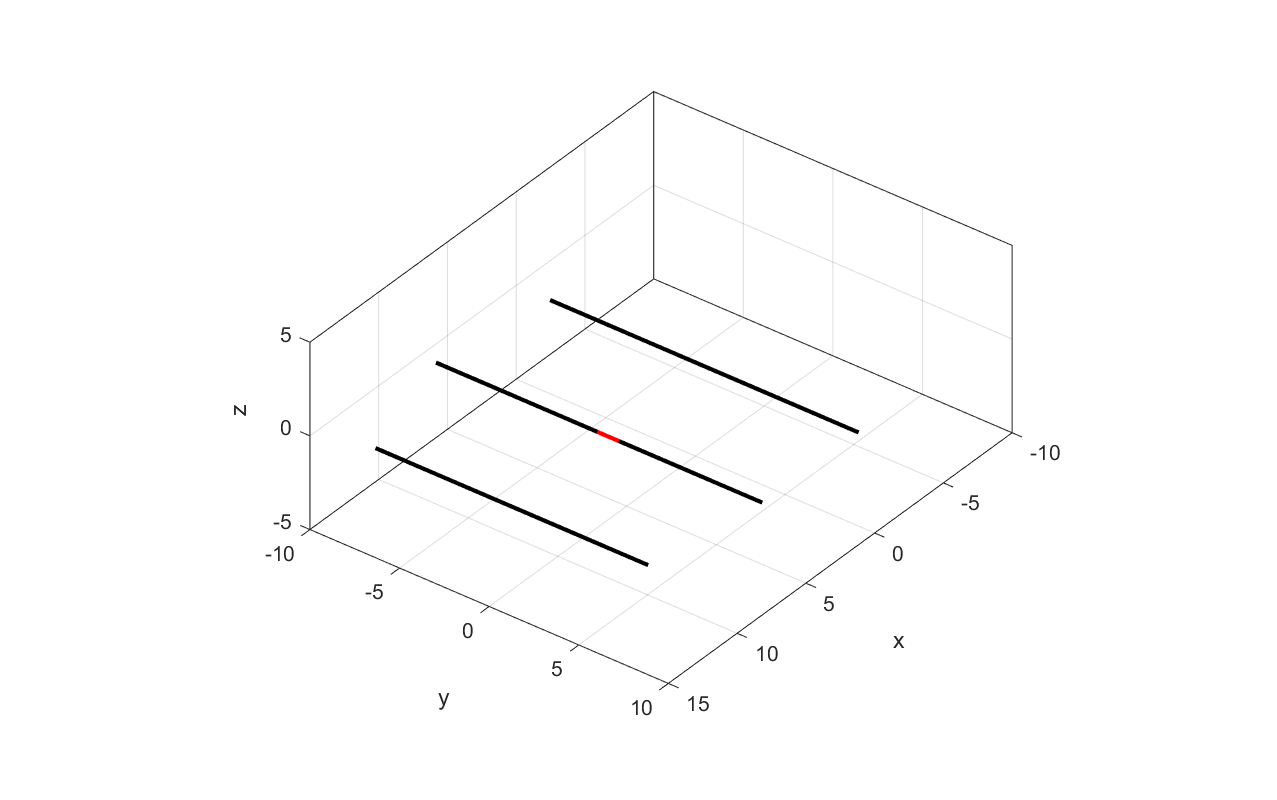
\includegraphics[width=10cm]{3_element_yagi-uda_geometry.eps}
  \caption{Figure showing the angles involved in the dipole inclination and rotation (WRITE SOURCE)}
  \label{fig:3_element_yagi-uda_geometry}
\end{figure}

\ptable{| p{12cm} | p{6cm} |}{ %
Parameter 		&	Value 			\\ \hline
Reflector size 		        &	$18 cells$	        \\ \hline
Dipole size 		        &	$16 cells$	        \\ \hline
Director size 		        &	$12 cells$	        \\ \hline
Reflector position (x axis) 		        &	$0 cells$	        \\ \hline
Dipole position (x axis) 		        &	$9 cells$	        \\ \hline
Director position (x axis) 		        &	$14 cells$	        \\ \hline
Cell size 		        &	$\SI{0.01}{\meter}$	        \\ \hline
Excitation lower freq 		        &	$\SI{1}{\hertz}$	        \\ \hline
Excitation higher freq 		        &	$\SI{1.7}{\giga\hertz}$	        \\ \hline
}{Simulation and design parameters}{tab:antenna_param}

From the radiation diagram of \figref{fig:yagi_radiation_pattern_director} we can see that the three elements Yagi-Uda antenna presents a gain of 6 dBi. These results are close to those found in a reference on-line for Yagi-Uda antennas (\figref{fig:3_element_yagi-uda}) where it is said that the gain of a 3-elements Yagi-Uda antenna is of 6.3 dBi.

\begin{figure}[!h]
  \centering
  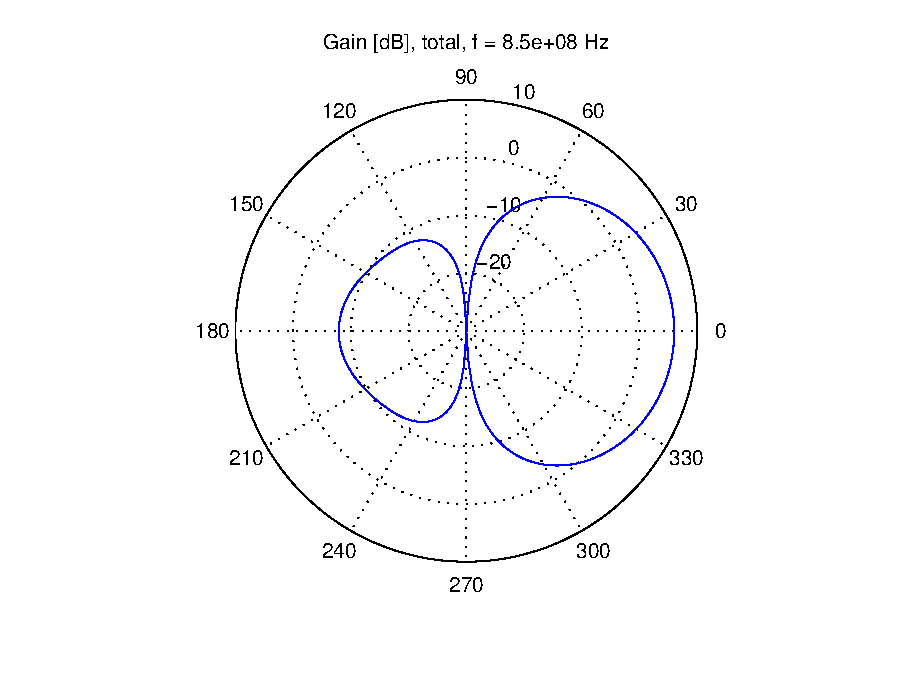
\includegraphics[width=10cm]{yagi_radiation_pattern_director.eps}
  \caption{Figure showing the angles involved in the dipole inclination and rotation (WRITE SOURCE)}
  \label{fig:yagi_radiation_pattern_director}
\end{figure}

\begin{figure}[!h]
  \centering
  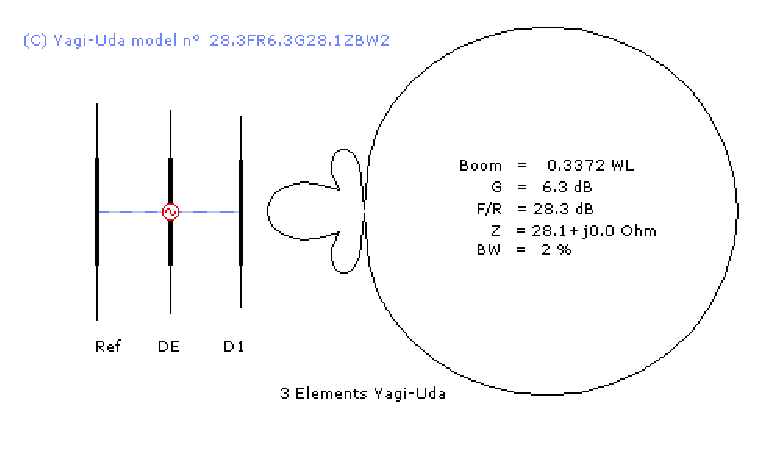
\includegraphics[width=10cm]{3_element_yagi-uda.eps}
  \caption{Figure showing the angles involved in the dipole inclination and rotation (WRITE SOURCE)}
  \label{fig:3_element_yagi-uda}
\end{figure}

For didactical purposes we tried to simulate the Yagi-Uda antenna without the director. The geometry of the simulation is shown in \figref{fig:2_element_yagi-uda_geometry}. The simulated radiation pattern is shown in \figref{fig:yagi_radiation_pattern} and it can be seen that, as it was expected, it is a less directive antenna (with a gain of 5 dBi) than the 3-elements Yagi-Uda.

\begin{figure}[!h]
  \centering
  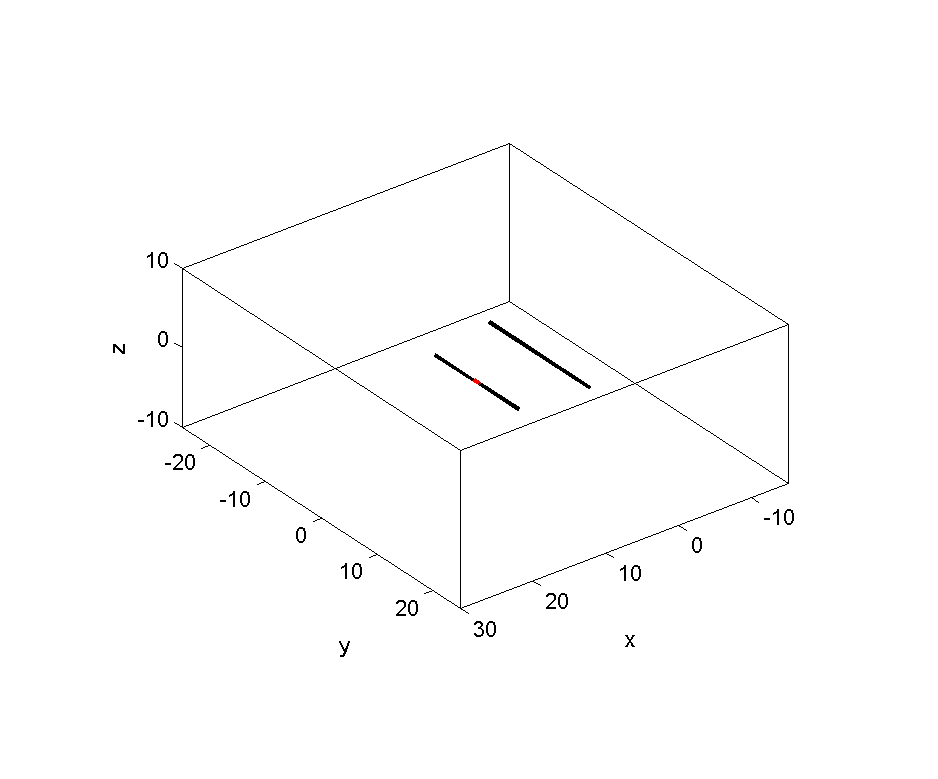
\includegraphics[width=10cm]{2_element_yagi-uda_geometry.eps}
  \caption{Figure showing the angles involved in the dipole inclination and rotation (WRITE SOURCE)}
  \label{fig:2_element_yagi-uda_geometry}
\end{figure}

\begin{figure}[!h]
  \centering
  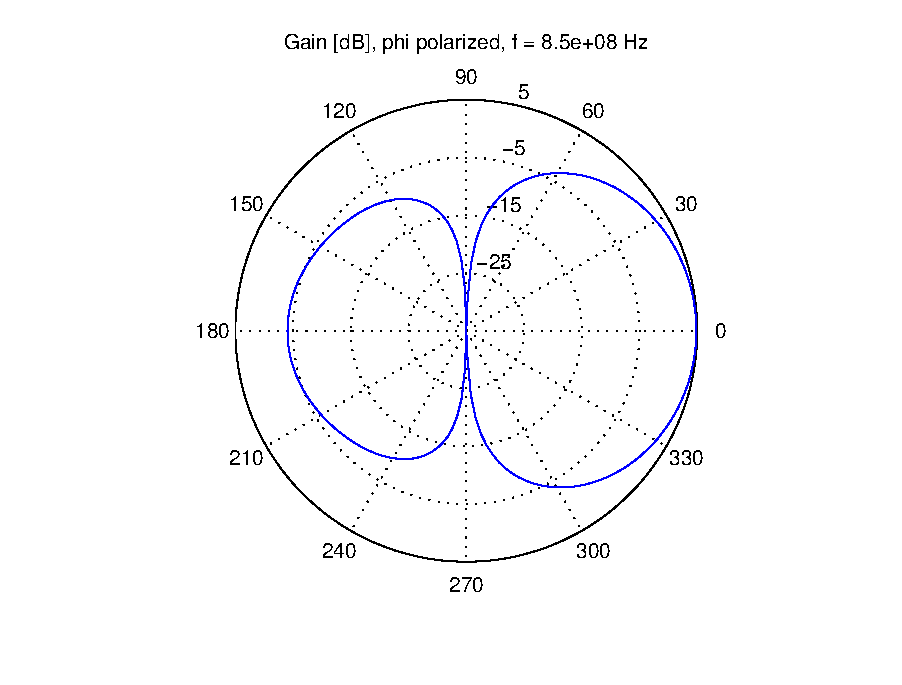
\includegraphics[width=10cm]{yagi_radiation_pattern.eps}
  \caption{Figure showing the angles involved in the dipole inclination and rotation (WRITE SOURCE)}
  \label{fig:yagi_radiation_pattern}
\end{figure}
